\documentclass{article}

\usepackage[utf8]{inputenc}
\usepackage[spanish]{babel}

\usepackage{geometry}               % Márgenes del documento
\usepackage{amsfonts}
\usepackage{graphicx}

\usepackage[nottoc]{tocbibind}

\usepackage{color}
\usepackage[pdftex, colorlinks=true, linkcolor=blue, urlcolor=red, filecolor=magenta, citecolor=blue]{hyperref}
\definecolor{gray97}{gray}{.97}
\definecolor{gray75}{gray}{.75}
\definecolor{gray45}{gray}{.45}


\usepackage{listings}
\usepackage[usenames,dvipsnames]{xcolor}
\colorlet{keyword}{blue!100!black!80}
\colorlet{STD}{Lavender}
\colorlet{comment}{green!80!black!90}

\lstdefinestyle{miniBash}{
	language     = bash,
	tabsize=3,
	numbers=left, % Donde se situan los numeros
	frame=none, % Se pone un marco
	showstringspaces=false, % No muestre el cuadrado en los espacios de los strings
	backgroundcolor = \color{gray97},
	basicstyle   = \footnotesize \ttfamily,
	keywordstyle = [1]\color{keyword}\bfseries,
	keywordstyle = [2]\color{STD}\bfseries,
	breaklines=true,                % sets automatic line breaking
	commentstyle = \color{comment}
}

\lstdefinestyle{C}{
	language     = C,
	tabsize=3,
	numbers=left, % Donde se situan los numeros
	frame=single, % Se pone un marco
	showstringspaces=false, % No muestre el cuadrado en los espacios de los strings
	backgroundcolor = \color{gray97},
	basicstyle   = \footnotesize \ttfamily,
	keywordstyle = [1]\color{keyword}\bfseries,
	keywordstyle = [2]\color{STD}\bfseries,
	breaklines=true,                % sets automatic line breaking
	commentstyle = \color{comment}
}

\geometry{a4paper}                  % Tamaño y márgenes del documento
\geometry{left=2.5cm,top=2.5cm}
\geometry{bottom=2.5cm,right=2.5cm}

\geometry{driver=dvips,pdftex} % ???
\setcounter{secnumdepth}{5}    % ???
\setcounter{tocdepth}{5}       % ???

\setlength{\parskip}{\baselineskip} % Espacio entre párrafos (una linea en blanco)

%--------------------------------------------------------------------------
\title{\textbf{Informática como servicio}
\\ \textbf{\emph{StarCluster}}
}
\author{Francisco Abel Cedrón Santaeufemia \and \textit{francisco.cedron@udc.es}}
\date{} %Asi no inserta la fecha

\addto\captionsspanish{
\def\tablename{Tabla}
\def\listtablename{Índice de tablas}
}

\begin{document}
\maketitle % Pone titulo, autor
\renewcommand{\abstractname}{Abstract} % El nombre que aparece al principio del abstract
\begin{abstract}
	En este documento se puede leer el trabajo realizado por el alumno para la práctica optativa de informática como servicio. El objetivo de este trabajo es poder mostrar con un código altamente paralelizable la importancia de disponer de una gran potencia de calculo empleando varias maquinas para la ejecucion de un programa. Ademas se implementara un sistema de colas de trabajo en el que se puedan poner procesos en una cola de ejecucion para ejecutarse de manera ordenada.
\end{abstract}
\renewcommand{\contentsname}{} % Lo que pone en el indice
{\setlength{\parskip}{0mm} \tableofcontents} % Para que no ponga espacios entre las lineas de indice
%\vspace{1cm} % Para dejar un espacio con respecto a la tabla

\section{Descripción de la práctica}
	El objetivo de esta práctica es poder crear un entorno para poder ejecutar programas paralelos con diversas máquinas. Para ello empezaremos por crearnos un programa paralelo para poder ver las ventajas de poder ejecutar programas en varias máquinas.
	
\section{Programa paralelo}
{\setlength{\parskip}{0mm}
	La aplicación que se desarrollo en estre trabajo es una manera de escalar una imagen digital. Dicho proceso se hace mediante la siguiente transformación:
\begin{equation}
R(x, y) = A \left( \frac{x}{i_x}, \frac{y}{i_y} \right)
\end{equation}
donde \emph{A(x, y)} es la imagen de entrada mientras que \emph{R(x, y)} es la salida y donde el valor de $i_x$ indica el incremento en el eje horizontal 
e $i_y$ el incremento en el eje vertical. El problema que puede ocasionar dicha transformación es que puede dar valores de números decimales en 
los índices con lo que intenta referenciar un valor de un pixel que no existe en una imagen. Para poder solucionar este problema se emplea la interpolación. 
Los métodos más comunes de interpolar una imagen son los siguientes:
\begin{enumerate} {\setlength{\parskip}{0mm}
	\item Interpolación por el vecino más próximo.
	\item Interpolación bilineal.
	\item Interpolación bicúbica.
} \end{enumerate}
}

	La interpolación por el vecino más próximo resuelve el problema cogiendo el valor del pixel más próximo, siendo una manera sencilla de implementar y con una rápida ejecución pero consigue un efecto pixelado en los resultados. Para poder mejorar los resultados obtenidos se puede emplear la interpolación bilineal que para obtener el valor de un pixel que no existe usa los cuatro reales que están a su alrededor y calcula una media ponderada consiguiendo así un mejor resultado visual en la imagen de salida, pero con un tiempo de ejecución mucho mayor. Si aún así se necesita unos mejores resultados se puede emplear una interpolación bicúbica que requiere el uso de 16 pixels. El resultado que se consigue con la interpolación bicúbica es eliminar los efectos ``cuadriculados'' que se obtienen empleando con la interpolación bilineal, efecto que se consigue al emplear 16 pixels en vez de 4 al calcular el valor de un pixel resultante (a pesar del gran coste computacional que eso conlleva). Para poder ver el resultado obtenido con los distintos tipos de interpolación se puede ver el resultado en la figura \ref{fig:interpolationExample}.

\begin{figure}[h]
  \centering
    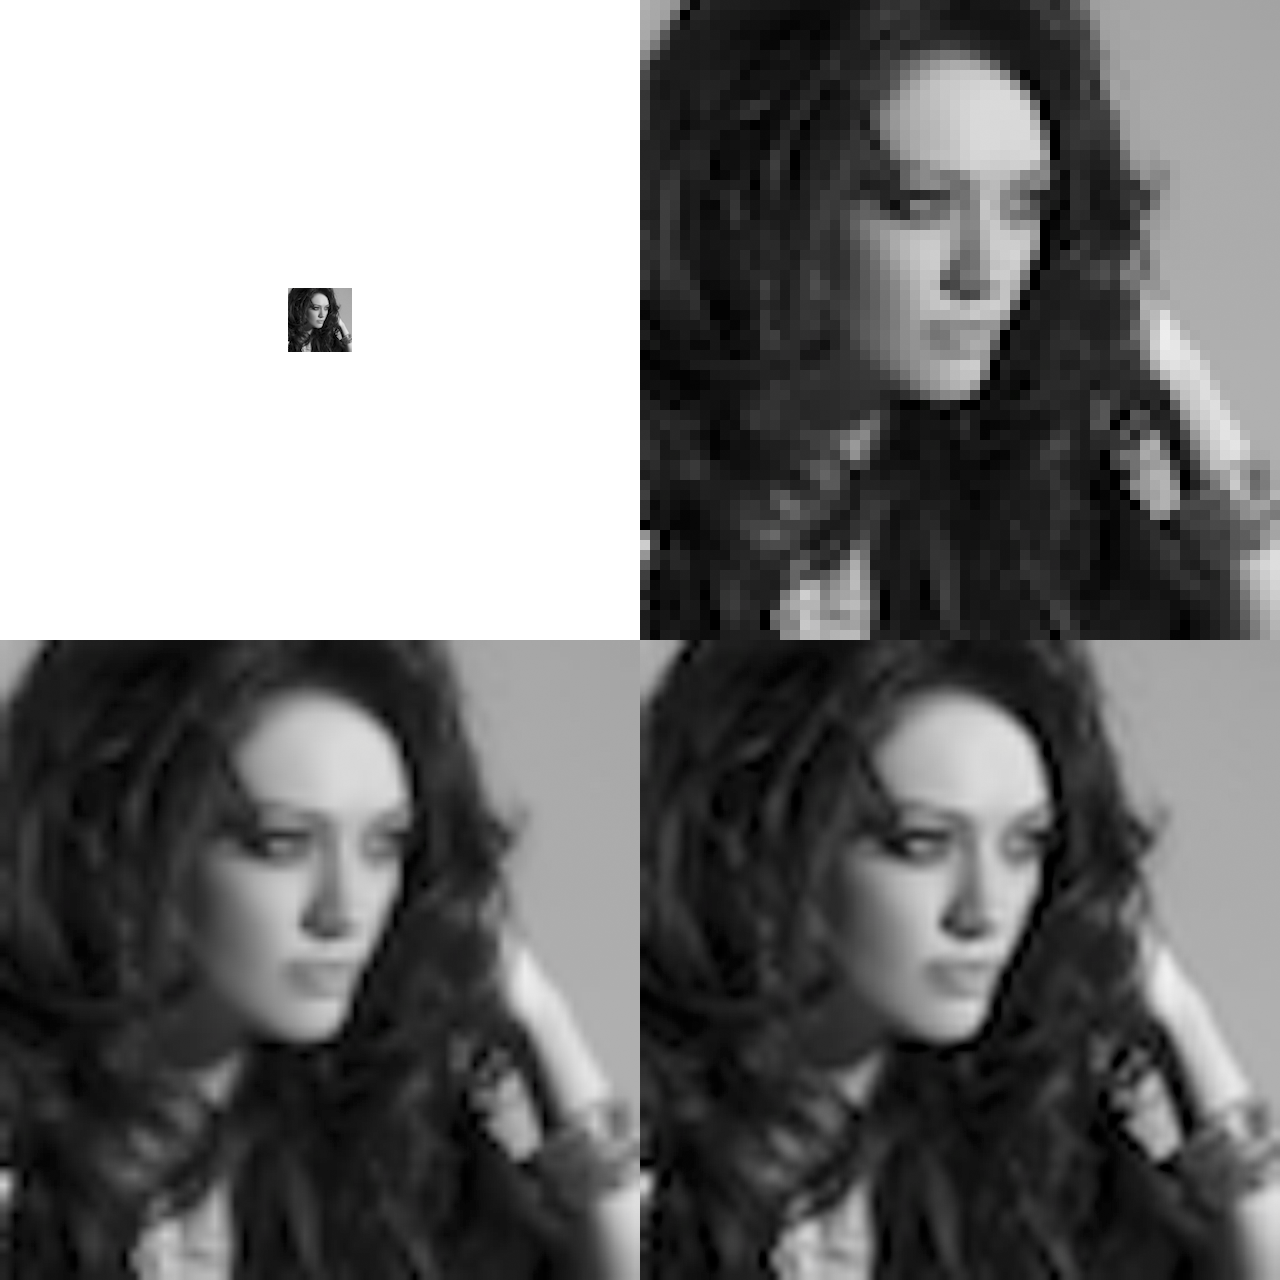
\includegraphics[width=0.5\textwidth]{img/example.png}
  \caption{Resultados obtenidos al emplear distintas interpolaciones. De izquierda a derecha y de arriba a abajo:
  a) imagen original, b) zoom 10x interpolación por vecino más próximo, c)zoom 10x interpolación bilineal, d) zoom 10x interpolación bicúbica.}
  \label{fig:interpolationExample}
\end{figure}

{\setlength{\parskip}{0mm}
El algoritmo que se desarrollará en este trabajo es el de interpolación bicúbica, que como hemos dicho emplea dos interpolaciones cúbicas. En el caso de una sola dimensión la interpolación cúbica consiste en trazar una cúbica entre los 4 puntos más próximos (2 a la izquierda y 2 a la derecha).
\begin{equation}
\label{eq:interpolacionCubica}
f(x) = c_0 x^3 + c_1 x^2 + c_2 x + c_3
\end{equation}
para aplicar la interpolación bicúbica se necesita hacer dos interpolaciones cúbicas:
\begin{enumerate}{\setlength{\parskip}{0mm}
	\item Interpolación cúbica \emph{horizontal}, en las filas existentes (usando 4 puntos).
	\item Interpolación cúbica \emph{vertical} en todo el espacio usando 4 puntos (empleando la anterior interpolación).
}\end{enumerate}
}

En este tipo de interpolación un punto \emph{($p_x$, $p_y$)} emplea 16 pixels circundantes. Así tenemos que el valor del punto se puede calcular como una media ponderada de los 4x4 pixels circundantes. Para calcular el punto interpolado hay que realizar
\begin{equation}
	A'(p_x ,p_y ) = \sum_{n = -1..2} \sum_{m=-1..2} A(i+n, j+m)P(n-a)P(b-m)
\end{equation}
siendo
\begin{displaymath}
	\begin{matrix}	
		P(k) = \frac{1}{6}(C(k+2)^3 - 4C(k+1)^3 + 6C(k)^3 -4C(k-1)^3) \\
		C(k) = max\lbrace 0, k \rbrace
	\end{matrix}
\end{displaymath}

\begin{figure}[h]
  \centering
    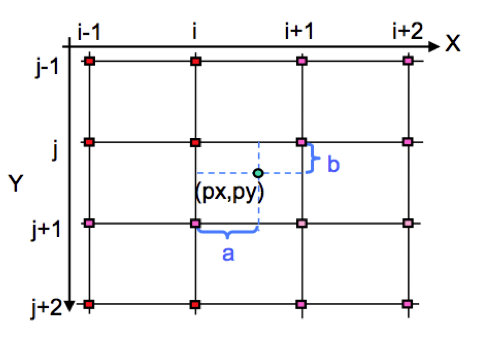
\includegraphics[width=0.45\textwidth]{img/interpolation.png}
  \caption{Parámetros empleados para realizar la interpolación bicúbica}
  \label{fig:interpolation}
\end{figure}



Un problema que hay que abordar en cuanto al uso del tipo de interpolación es saber qué pixels se van emplear en caso de que se necesite calcular valores que estén próximos al borde, para ello se pueden usar dos métodos:{\setlength{\parskip}{0mm}
\begin{enumerate}{\setlength{\parskip}{0mm}
	\item Usar ceros como valor siempre que se necesite un valor que esté fuere de la matriz de la imagen.
	\item Usar un efecto espejo en los bordes de la imagen.
}\end{enumerate}
}En este trabajo se implementará la segunda opción.

\subsection{Creación del programa}
Lo primero que se necesita es poder simular una imagen. Para ello se realiza una simulación tal y como se muestra en el siguiente trozo de código

\begin{lstlisting}[style=C]
void getImage(char *matrix, int height, int width) {
	int i,j;
	 
	for (i = 0; i < height; i++)
		for (j = 0; j < width; j++)
			matrix INDEX(i, j, width) = rand() % 256;//gray level
}
\end{lstlisting}

Al utilizar el método de escalado de una imagen descrito anteriormente nos encontraríamos con un problema al intentar hallar el valor de un pixel en los bordes de la imagen. Para solucionar este problema se llevó a cabo una de las soluciones encontradas en la literatura, se emplea el método de creación de bordes alrededor de la imagen con efecto espejo, añadiendo dos filas en la parte superior e inferior y también dos columnas a la izquierda y derecha de la imagen. 
En la figura \ref{fig:ejemploMatrices} se muestra un ejemplo representativo de la matriz original y la aumentada.

\begin{figure}[h]
\centering
\begin{lstlisting}
                               236  74  74 236  41 205 186 171 171 186
                               198 103 103 198 105 115  81 255 255  81 
  103 198 105 115  81 255      198 103 103 198 105 115  81 255 255  81   
   74 236  41 205 186 171      236  74  74 236  41 205 186 171 171 186
  242 251 227  70 124 194      251 242 242 251 227  70 124 194 194 124
   84 248  27 232 231 141      248  84  84 248  27 232 231 141 141 231
  118  90  46  99  51 159       90 118 118  90  46  99  51 159 159  51 
                                90 118 118  90  46  99  51 159 159  51
                               248  84  84 248  27 232 231 141 141 231	
\end{lstlisting}
\caption{Izquierda: Imagen original. Derecha: Imagen espejo.}
\label{fig:ejemploMatrices}
\end{figure}

Una vez que tenemos la imagen original y se han creado los ``bordes'', se realiza el proceso de escalado con la siguiente función

\begin{lstlisting}[style=C]
int ** getScale(char *mirror, char *result, int height, int width, int delay, float ix, float iy) {
	//Asignacion de memoria para la imagen resultante
	int **tmp = malloc(sizeof(int *)*(height*iy));
	
	if (tmp == NULL)
		exit_msg("getImage: cannot allocate memory (1)");
	
	int i,j;
	for (i = 0; i < height*iy; i++) {
		if ((tmp[i] = malloc(sizeof(int) * (width*ix))) == NULL)
			exit_msg("getImage: cannot allocate memory (2)");
	}

	int cnt = 0;
	int n, m;
	float sum;
	float pn, pm;
	float a, b;
	//Iniciar el proceso de convolucion
	for (i = 0; i < height*iy; i++) {//Bucle a paralelizar con MPI
		for (j = 0; j < width*ix; j++) {
			//tmp[i][j] = MAX(0, cnt++);
			sum = 0.0f;
			a = ((float) i)/ix  - ((int) i/ix);
			b = ((float) j)/iy  - ((int) j/iy);
			for (n = -1; n < 3; n++) { //Ambos bucles con SSE
				for (m = -1; m < 3; m++) {
					pn = Pk(n - a);
					pm = Pk(b - m);
					sum += mirror[(int) (i/ix+delay+n)][(int) (j/iy+delay+m)]*pn*pm;
				}
			}
			tmp[i][j] = (int) sum;	
		}
	}
	return tmp;
}
\end{lstlisting}

\subsection{Técnicas de paralelización utilizadas}
\subsubsection{Paso de mensajes con MPI}
Esta técnica se aplicó al bucle más externo. Con ella se pretendía dividir la carga computacional que crea este segmento de código entre varios procesadores, de manera que cada uno de ellos realizase una parte del cálculo, siendo así más rápida la terminación del programa. El motivo de realizar este reparto es dividir las filas de la imagen original para que cada proceso MPI se encargue de escalar su trozo de imagen tal y como se muestra en la figura \ref{fig:repartoFilas}.

\begin{figure}[h]
        \centering
        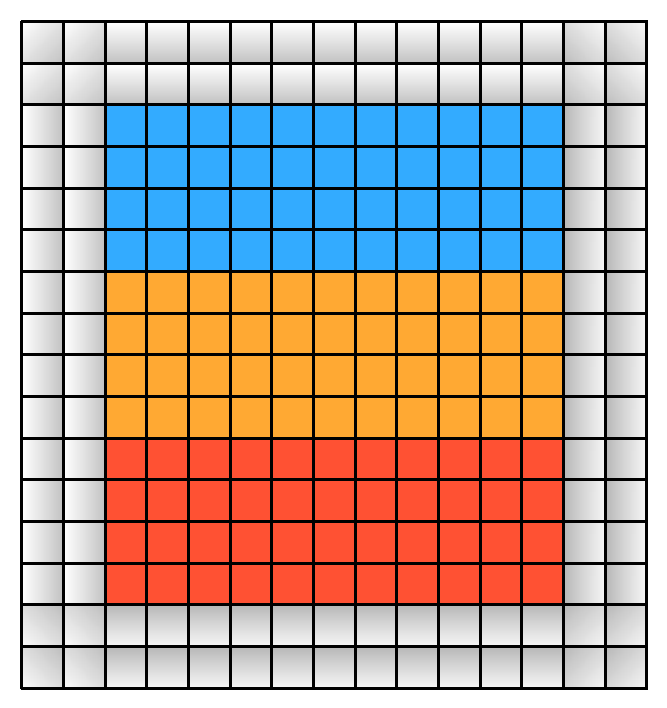
\includegraphics[angle=0, height=0.3\textheight]{img/repartoFilas.pdf}
        \caption{Imagen divida en filas. La región grisácea representa el espejo que se creo para dicha imagen. La imagen original esta formada por los píxels de color azul, naranja y rojo. Como se puede visualizar, la imagen está dividida en tres regiones, que son las que cada proceso MPI se encargaría de escalar.}
        \label{fig:repartoFilas}
\end{figure}

\begin{figure}[h]
        \centering
        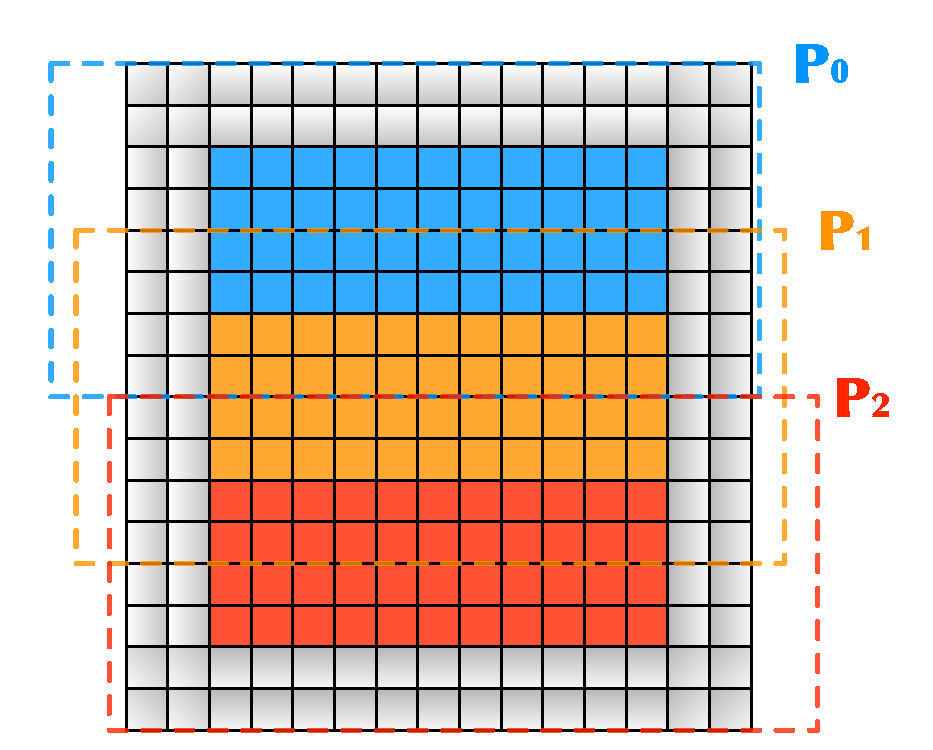
\includegraphics[angle=0, height=0.3\textheight]{img/repartoMPI.pdf}
        \caption{Cada color de la imagen original (azul, naranja o rojo) son las filas que tendrá que escalar cada proceso, pero para realizar el escalado necesita unos ``bordes'' para poder realizar la interpolación. Lo que se enviará a cada proceso MPI está delimitado con un rectángulo de líneas punteadas (mostrando así que hay trozos de la imagen que puede estar en varios procesos).}
        \label{fig:repartoMPI}
\end{figure}

Para poder repartir la matriz de la imagen entre los distintos procesos se utilizaron las funciones \emph{MPI\_Scatterv} y \emph{MPI\_Gatherv}. El motivo de su uso fue que los segmentos de matriz enviados a cada proceso estaban solapados, y estas funciones permiten indicar al padre en qué punto empieza la parte de la matriz que debe enviar a un proceso en concreto, así como el tamaño a enviar. Además este motivo fue la razón de que el reparto de trabajo fuese consecutivo, porque en el caso de ser cíclico, se tendría que enviar toda la imagen a todos los procesos. En la figura \ref{fig:repartoMPI} se puede ver como lo que se envía a cada proceso MPI está solapado con lo que se envía a otros procesos.

El motivo de tener que enviar a cada proceso partes solapadas de la matriz se explica por el mismo motivo de la creación de la matriz espejo, es decir, la parte que debe calcular cada proceso también tiene pixels en los ``bordes'', que necesitarán sus pixels circundantes para calcular su nuevo valor.

Para que se pueda repartir a cada proceso la información necesaria se debe poder indicar las variables necesarias para llamar a las funciones \emph{MPI\_Scatterv} y \emph{MPI\_Gatherv} (la figura \ref{fig:scatterGather} muestra dichas funciones), con lo que en la versión de programa paralelo se han creado unas funciones que indican a las funciones de envío y recepción de MPI los detalles necesarios. Esas funciones se pueden ver en la figura \ref{cod:fill_to_MPI}.

\begin{figure}[h]
\begin{lstlisting}[style=C]
MPI_Scatterv(mirror, size_send_child, aux_split,
	MPI_CHAR, work, size_send_child[myid],
	MPI_CHAR, 0, MPI_COMM_WORLD);
			
MPI_Gatherv(result, size_send_dad[myid], MPI_CHAR,
	scale, size_send_dad, aux_begin,
	MPI_CHAR, 0, MPI_COMM_WORLD);
\end{lstlisting}
\caption{Funciones \emph{MPI\_Scatterv} y \emph{MPI\_Gatherv}}
\label{fig:scatterGather}
\end{figure}

\begin{figure}[h]
\begin{lstlisting}[style=C]
#define MIN(x,y) ((x<y)?x:y)

//Funcion para indicar las filas con las que trabajara cada proceso
void fill_aux_rows(int *array, int size, int height, int delay) {
	int rows = height / size;	
	if (height % size != 0)
		rows++;
	
	int i;
	for (i = 0; i < size; i++)
		array[i] = MIN(rows, height-i*rows) + 2*delay;
}

//Funcion para conocer el numero de elementos a enviar a cada proceso
void fill_size_send_child(int *fill, int size, int *rows, int width, int delay) {
	int i;
	
	for (i = 0; i < size; i++)
		fill[i] = rows[i]* (width + 2*delay);
}

//Funcion para conocer desde donde se empieza a enviar a cada proceso
void fill_aux_split(int *fill, int size, int stride, int width, int delay) {
	int i;
	
	for (i = 0; i < size; i++) 
		fill[i] = i * (stride - (width + delay*2)*4);
}

//Funcion para conocer el tamano de la respuesta que enviara cada proceso
void fill_size_send_dady(int *fill, int size, int *rows, int width, float ix, float iy, int delay) {
	int i;
	
	for (i = 0; i < size; i++)
		fill[i] = (rows[i] -(2*delay))*iy * (width*ix);
}

//Funcion que indica al proceso que almacena el resultado donde tiene que colocar los resultados parciales
void fill_aux_begin(int *fill, int size, int bytes) {
	int i;
	
	for (i = 0; i < size; i++)
		fill[i] = bytes*i;
}
\end{lstlisting}
\caption{Funciones para necesarias para rellenar las variables que necesitan las variables que se pasan por parámetros a las funciones \emph{MPI-Gatherv} y \emph{MPI-Scatherv}}
\label{cod:fill_to_MPI}
\end{figure}

\end{document}